\subsection{Training}

The BDT training procedure, described in detail in
chapter~\ref{chap:bdt}, is performed after the common preselection and
the BJV. For \eemm events, the two \etmiss cuts are also applied
(track \etmiss~$>40$~\gev~and calo \etmiss~$>45$~\gev). The
CJV, OLV, and \Ztautaunody veto are not applied for training as these
cuts considerably decrease the background sample size, making it difficult for
the training algorithm to learn the kinematics of the
backgrounds. Moreover, a smaller training sample is more susceptible to
overtraining, a phenomenon in which the BDT has learned the
statistical or systematic fluctuations of the training sample and therefore does not
generalize to statistically independent samples
(section~\ref{chap:bdt:sec:decision_trees}).

The MC samples outlined in table~\ref{chap:analysis:tab:mc_summary} are used
in the training of the BDT. In order to use all of the available MC
statistics in the analysis, the cross-validation approach described
in section~\ref{subsec:cross_valid} is used. The training set is split
into two statistically independent samples-- even events and odd
events-- and a separate BDT is trained for each sample, yielding two
BDT functions: $F_{\textrm{even}}(\vect{x})$ and
$F_{\textrm{odd}}(\vect{x})$. For a given event, the BDT score is
obtained by applying the BDT that was trained on the orthogonal
training set, i.e.

 \begin{equation}
   \textrm{BDT}(\vect{x}_i) = \left\{
   \begin{array} {ll}
     F_{\textrm{even}}(\vect{x}_i) & \, \textrm{: event i is odd }
     \\
     F_{\textrm{odd}}(\vect{x}_i) & \, \textrm{: event i is even }
    \end{array} \right.
 \end{equation}

The background training sample is composed of all of the processes
listed in table~\ref{chap:analysis:tab:mc_summary}, with the exception of
\wjets and QCD. These two data-driven backgrounds are neglected, as
they include MC events with negative event weights, which are ignored
in the TMVA BDT implementation. The only Higgs process considered to
be signal in training is VBF. Given that the aim of the analysis is to
probe the signal strength of VBF, gluon fusion Higgs production is
treated as a background. Moreover, despite the fact that the $V$H
processes are considered signal in the likelihood fit, in the BDT
training they are ignored. Due to the negligible contribution of these
processes in the \lnln channel, the impact of removing them in the
training is small. 

Ascertaining the level of overtraining for the BDT is done by plotting
the BDT response distribution $F(\vect{x})$ for two statistically
independent samples. Disagreement in the shape is evidence of
overtraining. A comparison of the $F_{\textrm{even}}(\vect{x})$ distributions for the
training set (even events) and the test set (odd events) is
shown in Figure~\ref{chap:analysis:fig:overtraining1}, and
$F_{\textrm{odd}}(\vect{x})$ is shown in
Figure~\ref{chap:analysis:fig:overtraining2}. Signal, shown
in red, peaks close to a BDT score of 1, and background in blue peaks
at -1. The event yields are scaled to luminosity, with signal enhanced
by a factor of 50. Because background peaks so sharply at -1, the
first two background bins are scaled down by 20 and 2,
respectively. The Kolmogorov-Smirnov goodness-of-fit test is used to
quantify the level of agreement of the BDT response between the two
subsamples. In this test, the null hypothesis is that the two
distributions have the same underlying shape. For $F_{\textrm{even}}(\vect{x})$, the signal
(background) $p$-value is 0.021 (1.00) and for $F_{\textrm{odd}}(\vect{x})$, the $p$-values
are 0.122 (0.96). These $p$-values indicate that there is some degree
of overtraining for the signal. Looking at
Figure~\ref{chap:analysis:fig:overtraining}, the discrepancy
between the two subsamples lies at low BDT values, a phase space
region that is ultimately cut away in the analysis, as it does not
contribute any sensitivity. Moreover, because the
same BDT function is applied to the signal prediction, background
prediction, and the actual collision data, overtraining will not
invalidate the statistical results of an analysis; it can only result
in a suboptimal BDT.

\begin{figure}[h]
    \centering
    \subfigure[Overtraining check for BDT 1]{
    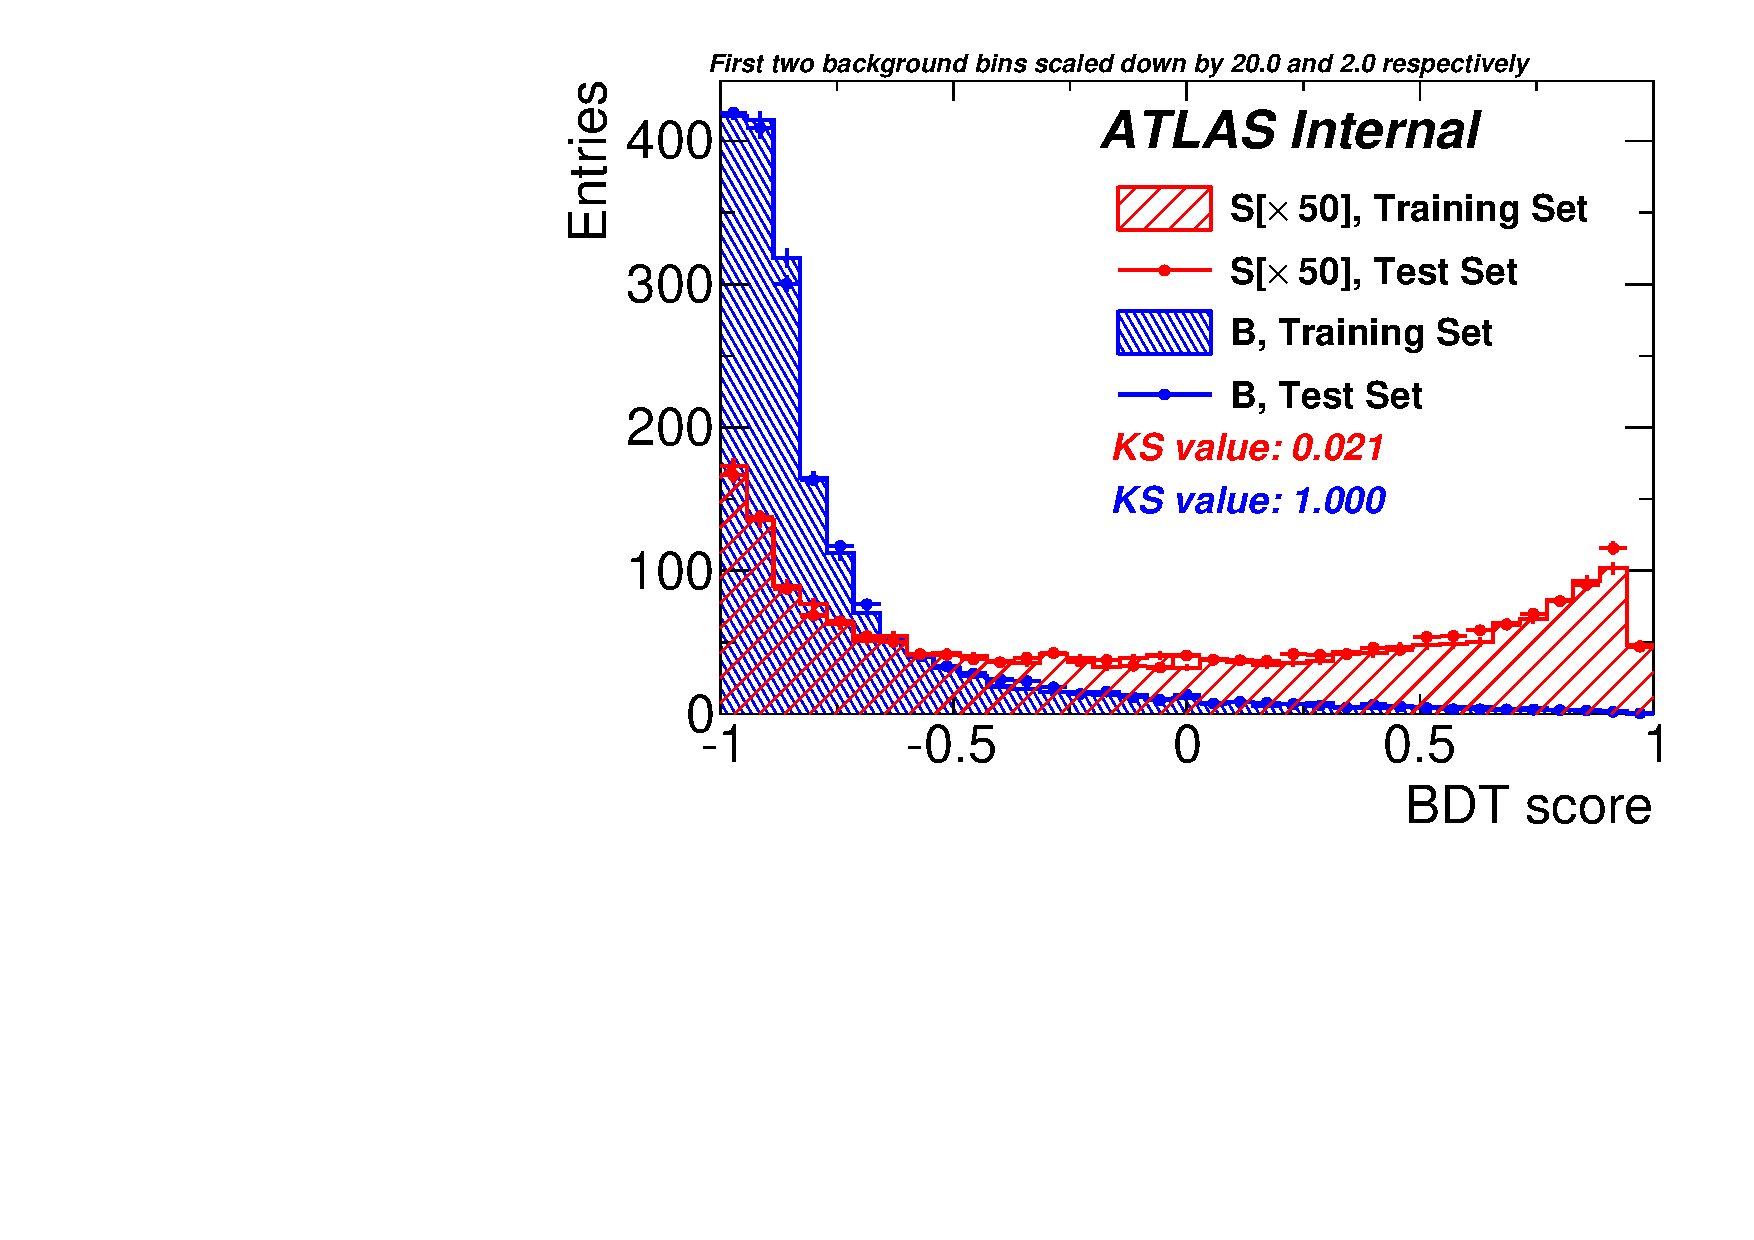
\includegraphics[width=0.45\textwidth]{bdt/overtraining_check1.pdf}
    \label{chap:analysis:fig:overtraining1}
    }
    \subfigure[Overtraining check for BDT 2]{
    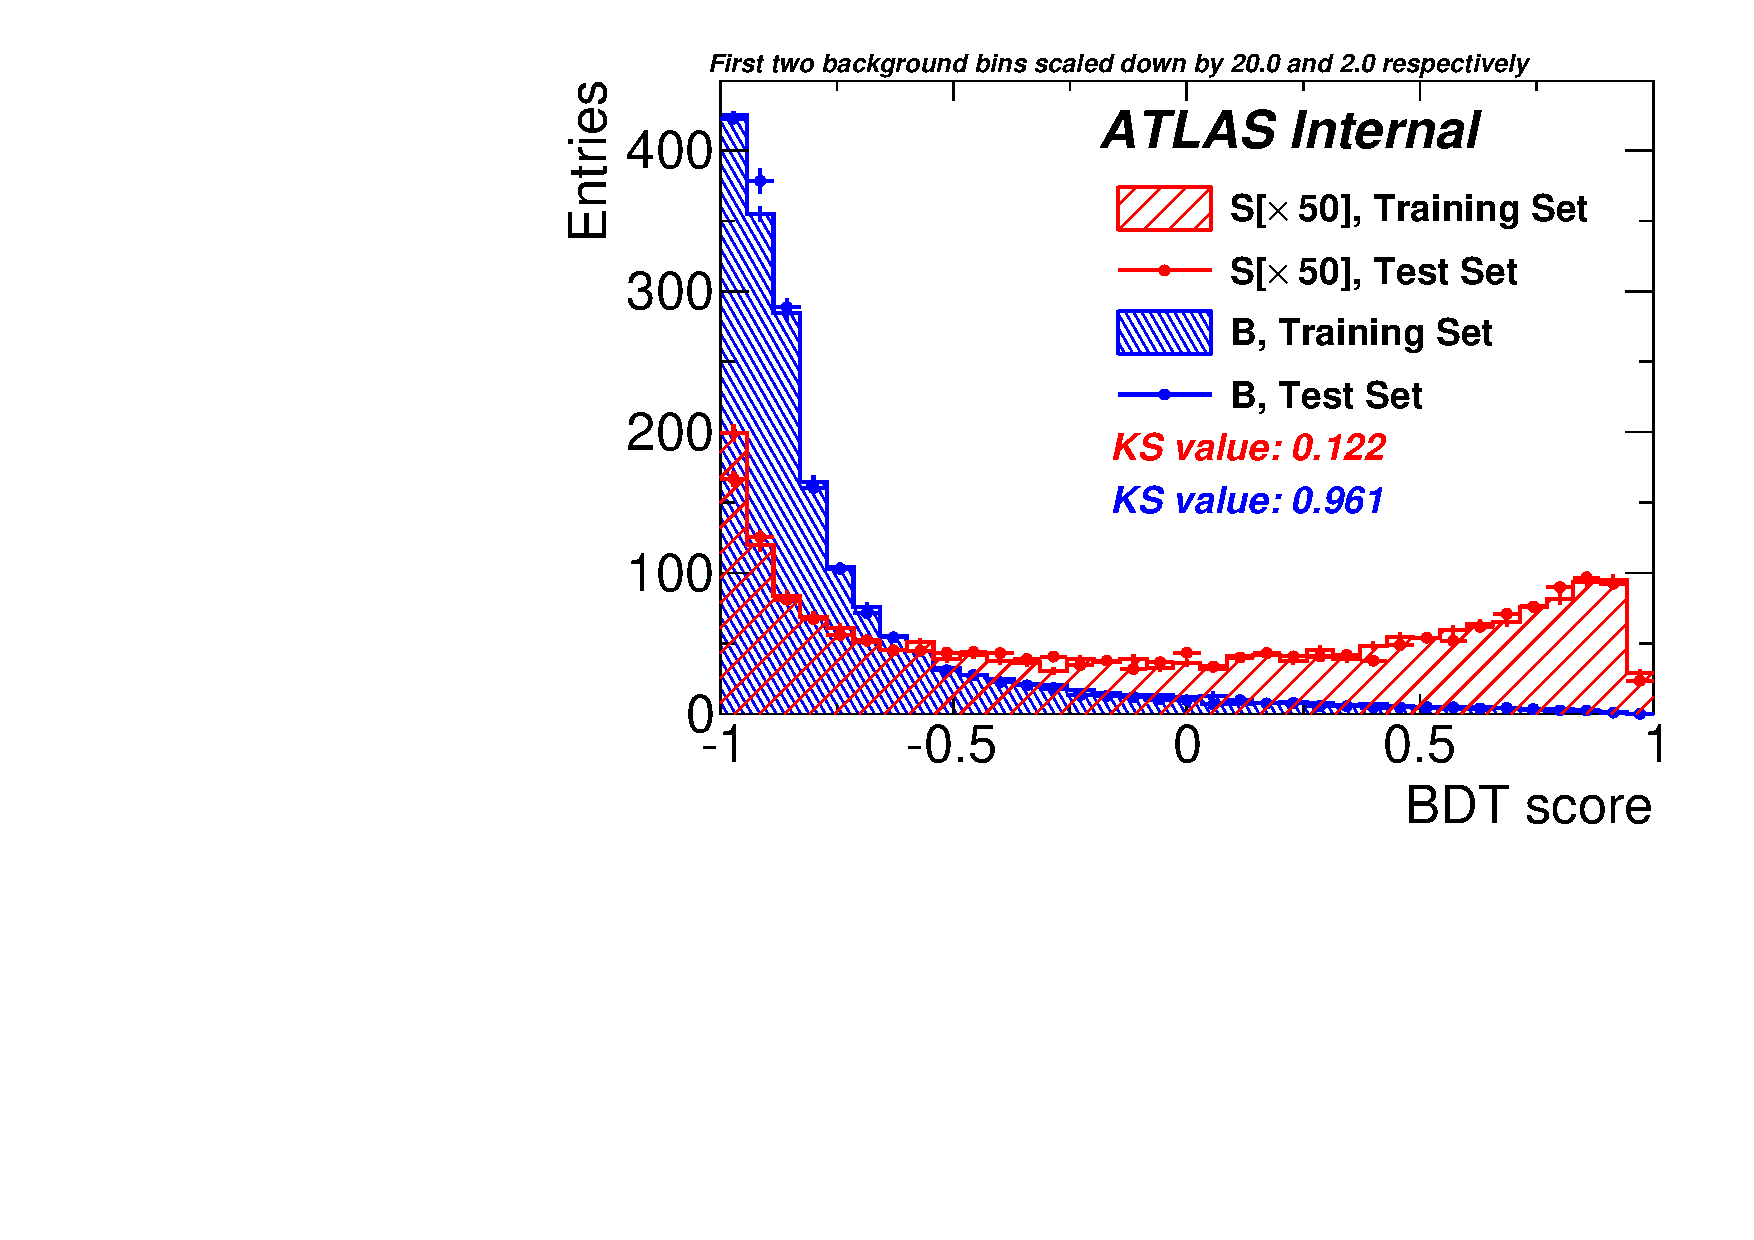
\includegraphics[width=0.45\textwidth]{bdt/overtraining_check2.pdf}
    \label{chap:analysis:fig:overtraining2}
    }
    \caption[Boosted decision tree overtraining check.]{Overtraining
      check for the optimized boosted decision tree. Training sets are shown
    with hatched distributions, while the statistically independent test sets
    are shown with points. The first two background bins are scaled
    down by factors of 20 and 2, respectively, in order to illustrate
    agreement at high BDT values. Morever, the signal normalization is multiplied by a factor
    of 50.}
\label{chap:analysis:fig:overtraining}
\end{figure}

\subsection{Data-MC Comparisons}

The BDT training relies on MC simulation to model the shapes of, and
the correlations among, the BDT inputs. In order to validate the
modeling, the level of agreement between data and MC in the BDT input
distributions is quantified in signal-depleted validation
regions. There are three such regions in this analysis: a low BDT
region, a top-rich region, and a \ZDY-rich region. The latter two will
be discussed in sections~\ref{} and~\ref{}, respectively. 

The low BDT validation region has the same preselection cuts as the signal
region, with an additional cut on the BDT score-- $\textrm{BDT} < -0.48$. The cut
value for this region has been determined through a binning optimization
algorithm for the BDT distribution. Binning optimization is performed
on the BDT distribution because the binned likelihood fit is performed
on this distribution. Hence, the statistical sensitivity of the analysis is highly
sensitive to the choice of binning. A crucial consideration in the
optimization of binning is over-fitting on statistical
fluctuations. If the metric for statistical sensitivity is not
prudently chosen, sensitivity can be arbitrarily inflated
with ever-finer binning, as backgrounds fluctuate out of signal-rich
bins. Moreover, if there is over-fitting in the binning optimization,
and bins become entirely depleted of background, then systematic
uncertainties are not properly accounted for in the fit algorithm,
again resulting in an optimistic estimate of the statistical
sensitivity. 

The binning optimization algorithm for the BDT distribution has been
chosen to account for the above considerations. First, the
preselection cuts are applied and the BDT distribution is computed for
signal at $m_{\textrm{H}} = 125$~\gev, as well as all of the
backgrounds. Because BDT peaks sharply at one for signal, the
algorithm starts at the right side of the BDT distribution, and in
BDT steps of 0.02, integrates to the left. At each step, the Poisson
significance estimate, given by

\begin{equation}
\label{chap:analysis:equation:pois_sig}
Z_{\textrm{Pois}}(S,B) = \sqrt{2((S+B)\log{(1+S/B)}-S)},
\end{equation}

\noindent
where $S$ ($B$) is the signal (background) event count normalized to
luminosity, is computed. When a maximum in $Z_{\textrm{Pois}}(S,B)$ is
reached, the event yield for each background is checked, and if each
background is represented, a bin boundary is set at that BDT
value. The next iteration then begins at the new boundary until another
maximum is found. The procedure continues until the maximum
$Z_{\textrm{Pois}}(S,B)$ falls below some threshold as the integration
nears the background-dominant low BDT region. The significance curves
obtained in this procedure are shown in
figure~\ref{chap:analysis:fig:bin_opt}. The resulting bin boundaries
are -0.48, 0.3, and 0.78. The region BDT~$<-0.48$ is dominated by
background (in \emme, $B \sim 660$), with little signal (in \emme, $S \sim 5$),
and is consequently not included in the signal region. Instead, this
region is used to validate the modeling of BDT inputs. 

\begin{figure}[h]
  \centering
  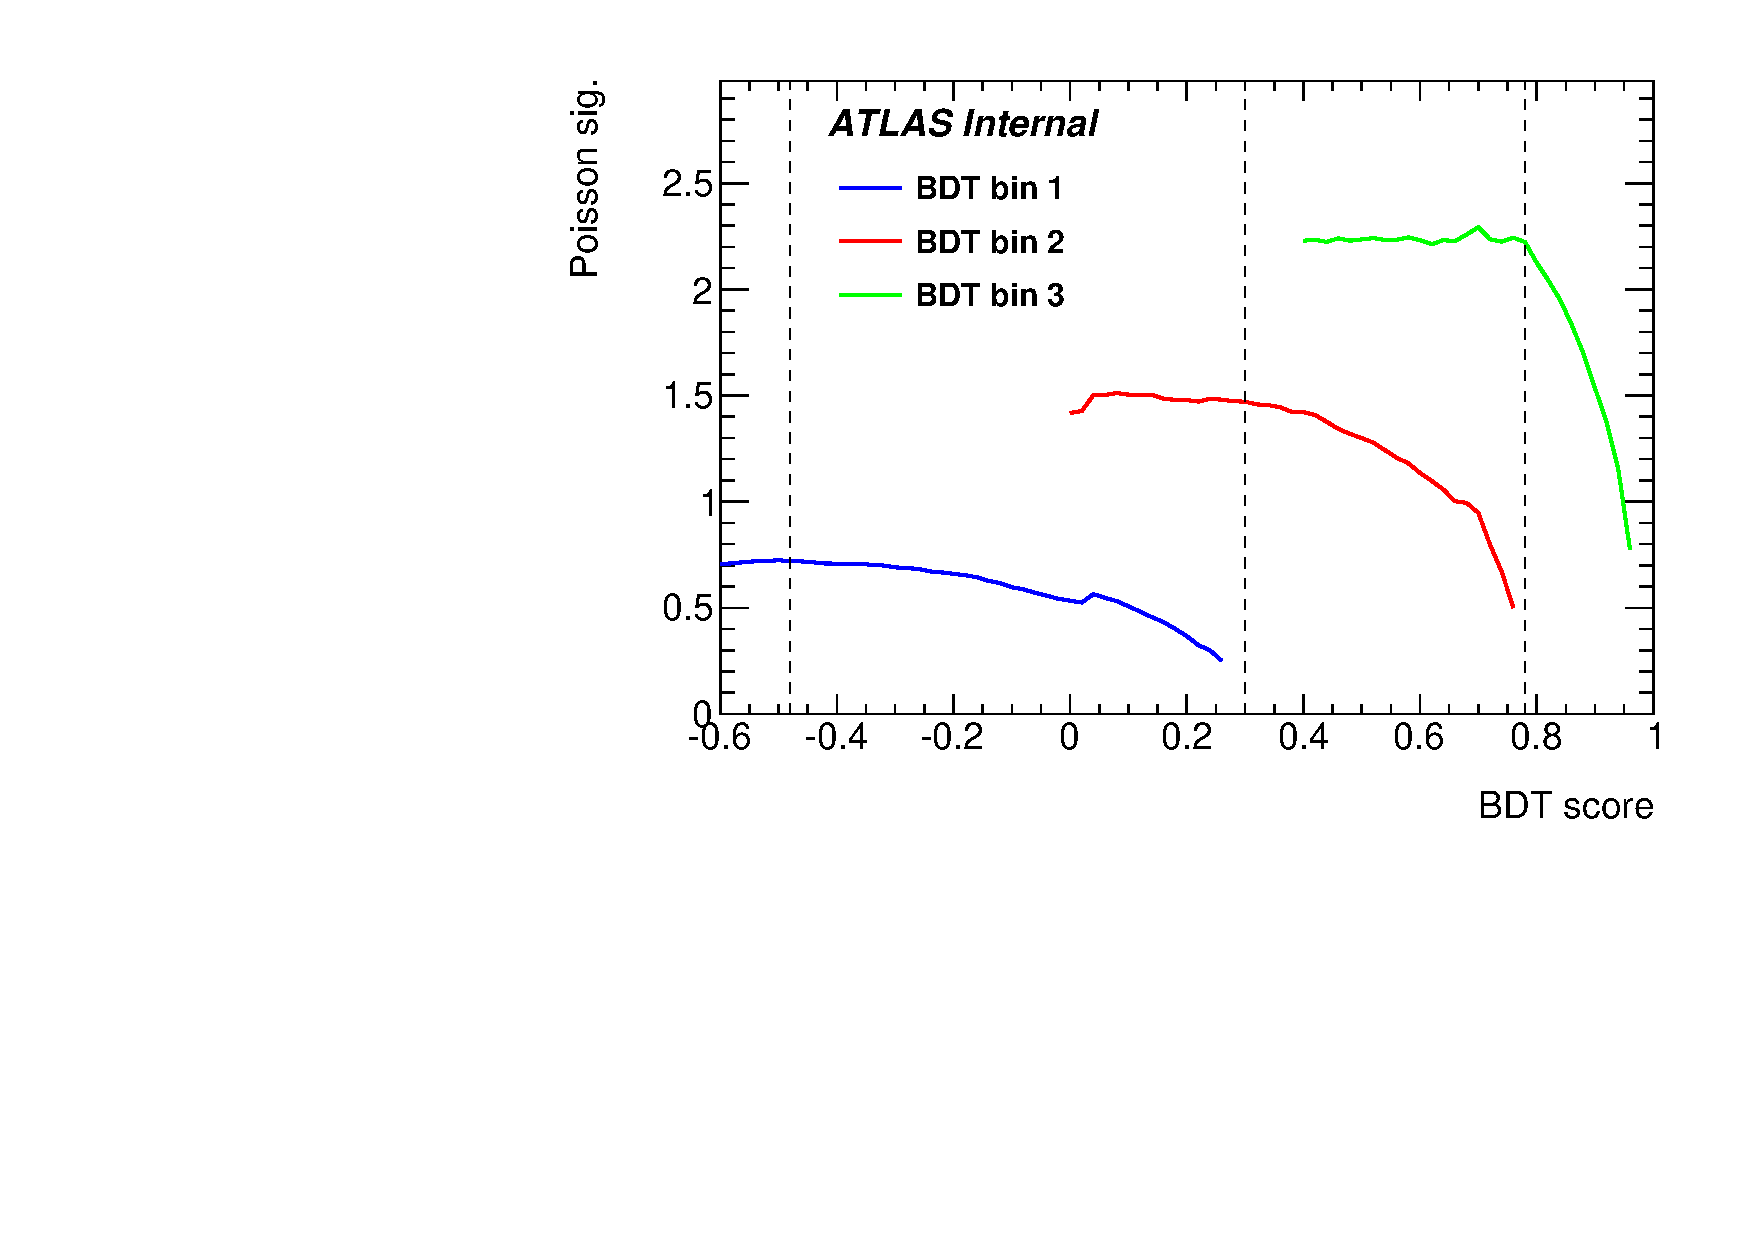
\includegraphics[width=0.6\textwidth]{fig/analysis/bin_opt_plot.pdf}
  \caption{Poisson significance scans used in the BDT bin optimization
  procedure. The resulting bin boundaries are shown as dashed lines:
  [-0.48,0.3,0.78]. Events falling in the region
  $\textrm{BDT} < -0.48$ are not included in the SR. Instead, this
  region is used to validate the modelling of the BDT inputs.}
  \label{chap:analysis:fig:bin_opt}
\end{figure}

Data-MC comparisons for the eight BDT inputs in the BDT~$<-0.48$
validation region (VR) are shown in
figure~\ref{chap:analysis:fig:low_bdt_vr_df}. Despite the fact that
there are not any data-driven corrections applied to the MC
predictions in these plots, the MC models the data well in this
region, as indicated by the $p$-value from the KS test for each BDT
input. The lowest $p$-value, for \lepEtaCent, is 0.38-- less than a
one sigma discrepancy. 

\begin{figure}[p!]
  \centering
  \includegraphics[width=0.4\textwidth]{fig/analysis/low_bdt_vr/emme_CutBDTScore_Bin1_DPhill_mh125_lin.eps}
   \includegraphics[width=0.4\textwidth]{fig/analysis/low_bdt_vr/emme_CutBDTScore_Bin1_Mll_mh125_lin.eps}
   \includegraphics[width=0.4\textwidth]{fig/analysis/low_bdt_vr/emme_CutBDTScore_Bin1_DYjj_mh125_lin.eps}
   \includegraphics[width=0.4\textwidth]{fig/analysis/low_bdt_vr/emme_CutBDTScore_Bin1_Mjj_mh125_lin.eps}
   \includegraphics[width=0.4\textwidth]{fig/analysis/low_bdt_vr/emme_CutBDTScore_Bin1_Pttot_tr_mh125_lin.eps}
   \includegraphics[width=0.4\textwidth]{fig/analysis/low_bdt_vr/emme_CutBDTScore_Bin1_MT_tr_mh125_lin.eps}

   \includegraphics[width=0.4\textwidth]{fig/analysis/low_bdt_vr/emme_CutBDTScore_Bin1_SumOFMvaMLepxJety_mh125_lin.eps}
   \includegraphics[width=0.4\textwidth]{fig/analysis/low_bdt_vr/emme_CutBDTScore_Bin1_contOLV_mh125_lin.eps}
   \caption{Distributions of the eight BDT inputs \dphill, \mll, \dyjj, \mjj, \pTtot,  \mT,
     \SumMlj, and \lepEtaCent in the \emme validation region (BDT
     score~$<-0.48$). Error band represents statistical
     uncertainties. Data-driven corrections to \ttbar~and \ZDY are not applied.}
  \label{chap:analysis:fig:low_bdt_vr_df}
\end{figure}

In addition to the one-dimensional BDT input distributions, the
modeling of the correlations among the BDT inputs has been
investigated. This is accomplished by plotting the average value of
the $i^{\textrm{th}}$ BDT input against the $j^{\textrm{th}}$ input
for all possible pairs of BDT inputs. The resulting matrix of
plots is shown in figure~\ref{chap:analysis:fig:bdt_corr_vr} for the
low BDT VR. The background color in each subplot is based on the
$p$-value for the $\chi^2$ test. If the $p$-value falls below 0.05,
the background is set to red. In this region, the MC models the correlations observed in
data well. Mis-modeling in the correlations will also manifest as
data-MC discrepancies in the BDT response distribution. 

\begin{figure}[h]
  \centering
  \includegraphics[width=1.0\textwidth]{fig/analysis/bdt_correlation_validation/correlations_PROF_lowBDT_VR.eps}
  \caption{Correlation plots of BDT inputs in the low BDT VR. Distributions of
    $< X_i >$ vs $X_j$ are shown for each BDT input pair. Data is
    shown in black, while the MC prediction for the background is in
    red. The background color for a given plot is set according to the
  $p$-value from the $\chi^2$ test. If the $p$-value is less than
    0.05, i.e. the discrepancy is greater than 2$\sigma$, the
    background is red. The test only accounts for statistical uncertainties.}
  \label{chap:analysis:fig:bdt_corr_vr}
\end{figure}

